% Copyright (c) 2017-2019 Matematyka dla Ciekawych Świata (http://ciekawi.icm.edu.pl/)
% Copyright (c) 2017-2019 Robert Ryszard Paciorek <rrp@opcode.eu.org>
% 
% MIT License
% 
% Permission is hereby granted, free of charge, to any person obtaining a copy
% of this software and associated documentation files (the "Software"), to deal
% in the Software without restriction, including without limitation the rights
% to use, copy, modify, merge, publish, distribute, sublicense, and/or sell
% copies of the Software, and to permit persons to whom the Software is
% furnished to do so, subject to the following conditions:
% 
% The above copyright notice and this permission notice shall be included in all
% copies or substantial portions of the Software.
% 
% THE SOFTWARE IS PROVIDED "AS IS", WITHOUT WARRANTY OF ANY KIND, EXPRESS OR
% IMPLIED, INCLUDING BUT NOT LIMITED TO THE WARRANTIES OF MERCHANTABILITY,
% FITNESS FOR A PARTICULAR PURPOSE AND NONINFRINGEMENT. IN NO EVENT SHALL THE
% AUTHORS OR COPYRIGHT HOLDERS BE LIABLE FOR ANY CLAIM, DAMAGES OR OTHER
% LIABILITY, WHETHER IN AN ACTION OF CONTRACT, TORT OR OTHERWISE, ARISING FROM,
% OUT OF OR IN CONNECTION WITH THE SOFTWARE OR THE USE OR OTHER DEALINGS IN THE
% SOFTWARE.

\documentclass{pdfBooklets}

\title{Zestaw do zajęć praktycznych z elektroniki}
\author{%
	Projekt ,,Matematyka dla Ciekawych Świata'',\\
	Robert Ryszard Paciorek\\\normalsize\ttfamily <rrp@opcode.eu.org>
}
\date  {2020-04-08}

\makeatletter\hypersetup{
	pdftitle = {\@title}, pdfauthor = {\@author}
}\makeatother

\usepackage[ampersand]{easylist}

\newcommand\zaleta{\item[\textbf{\ttfamily +}]}
\newcommand\wada{\item[\textbf{\ttfamily -}]}
\newcommand\info{\item[\textbf{\ttfamily *}]}
\newcommand\uwaga{\item[\textbf{\ttfamily !}]}

\begin{document}

\maketitle

\section{Zasilacz}
	Jednym z najważniejszych elementów zestawu służącego do zabawy elektroniką jest źródło zasilania.
	Może nim być nawet zwykła bateria, jednak dla wygody i bezpieczeństwa podłączanych układów warto posiadać podstawowy zasilacz regulowany z regulowanym ograniczeniem prądowym.
	Powinien on zapewniać co najmniej:
	\begin{itemize}
		\item regulację napięcia wyjściowego w zakresie od 2.5V do 7V
		\item regulowane ograniczenie prądowe\footnote{
			w przypadku próby pobrania większego prądu niż nastawiony zasilacz powinien
			przejść z trybu stałego napięcia (CV) do trybu stałego prądu (CV)
			i obniżyć podawane napięcie tak aby płynął nastawiony prąd.
		} w zakresie od 20mA do 500mA
		\item sygnalizacja trybu CV/CC (np. za pomocą diody LED)
	\end{itemize}
	Dla wygody jego używania warto aby był wyposażony także w:
	\begin{itemize}
		\item woltomierz pokazujący wartość napięcia wyjściowego
		\item amperomierz pokazujący wartość prądu podawanego do obciążenia
	\end{itemize}
	
	\subsection{Propozycje}
	
	\subsubsection{przetwornica DC/DC Step-Down XL4015}
		\begin{center}
			\includegraphics[height=3.3cm]{warsztat_elektroniczny/moduł_XL4015_1}
		\end{center}
		\begin{itemize}
			\wada brak zabezpieczenia przed odwrotną polaryzacją zasilania wejściowego (zamianą plusa z minusem na wejściu)
			\wada brak wskazań wartości napięcia i prądu
			\info od 8PLN (moduł "czerwony"), od 10PLN (moduł "niebieski")
			\uwaga należy zwrócić uwagę aby moduł posiadał dwa potencjomery - jeden do regulacji napięcia drugi prądu (występują moduły umożliwiające tylko regulację napięcia)
		\end{itemize}
	
	\subsubsection{przetwornica DC/DC Step-Down XL4015 z woltomierzem i amperomierzem LED}
		\begin{center}
			\includegraphics[height=3.3cm]{warsztat_elektroniczny/moduł_XL4015_LED_1}
			\hspace{0.5cm}
			\includegraphics[height=3.3cm]{warsztat_elektroniczny/moduł_XL4015_LED_2}
		\end{center}
	
		\begin{itemize}
			\zaleta modularna konstrukcja (oparta na opisanym wcześniej module "czerwonym")
			\wada brak zabezpieczenia przed odwrotną polaryzacją zasilania wejściowego (zamianą plusa z minusem na wejściu)
			\wada mała dokładność pomiaru (wskazuje 0.01A gdy płynie 0.1A)
			\wada brak możliwości (oficjalnie udokumentowanej) kalibracji pomiarów
			\wada słaba czytelność wyświetlacza LED przy dobrym oświetleniu
			\info od 30PLN
		\end{itemize}
		
	\subsubsection{przetwornica DC/DC Step-Down XL4015 z woltomierzem i amperomierzem LCD}
		\begin{center}
			\includegraphics[height=3.3cm]{warsztat_elektroniczny/moduł_XL4015_LCD_1}
			\hspace{0.5cm}
			\includegraphics[height=3.3cm]{warsztat_elektroniczny/moduł_XL4015_LCD_2}
			\hspace{0.5cm}
			\includegraphics[height=3.3cm]{warsztat_elektroniczny/moduł_XL4015_LCD_3}
		\end{center}
		\begin{itemize}
			\zaleta  zabezpieczenie przed odwrotną polaryzacją zasilania wejściowego (zamianą plusa z minusem na zaciskach wejściowych),
				\textbf{uwaga:} dotyczy wersji pokazanej na zdjęciu, podobna wersja z dwoma dodatkowymi LEDami najprawdopodobniej nie posiada tego zabezpieczenia
			\zaleta  dobra precyzja pomiaru (wskazuje 0.04A gdy płynie 0.03A)
			\zaleta  możliwość łatwej kalibracji pomiarów
			\wada niebezpieczne gniazdko USB (można podać na nie zbyt wysokie napięcia)
			\info od 40PLN
		\end{itemize}
		
	\subsubsection{elementy dodatkowe}
	Do wybranej przetwornicy sugerujemy dokupienie gniazda DC 2.5/5.5 wraz z przewodem oraz baterii 9V (ze złączem i wtykiem DC 2.5/5.5) lub zasilacza wtyczkowego np. 12V z prądem większym niż 0.9A (z wtykiem DC 2.5/5.5). Pozwoli to na wygodne podłączanie i odłączanie zasilania od przetwornicy poprzez rozpięcie wtyku DC.
	\begin{center}
		\includegraphics[height=4.3cm]{warsztat_elektroniczny/przewody_zasilające}
	\end{center}

\section{Multimetr}
	Najważniejszym przyrządem w naszym warsztacie elektronika jest uniwersalny miernik parametrów elektrycznych, zwany multimetrem.
	Dla naszych potrzeb powinien on zapewniać co najmniej:
	\begin{itemize}
		\item pomiar napięcia stałego (DC) od 0.1V do 20V (np. zakresy pomiarowe: 200mV, 20V)
		\item pomiar prądu stałego (DC) od 1mA do 200mA (np. zakresy pomiarowe: 20mA, 200mA)
		\item pomiar rezystancji od 10Ω do 1MΩ (np. zakresy pomiarowe: 200Ω, 20kΩ, 2000kΩ)
		\item pomiar diody
	\end{itemize}
	
	\begin{wrapfigure}{r}{6.5cm}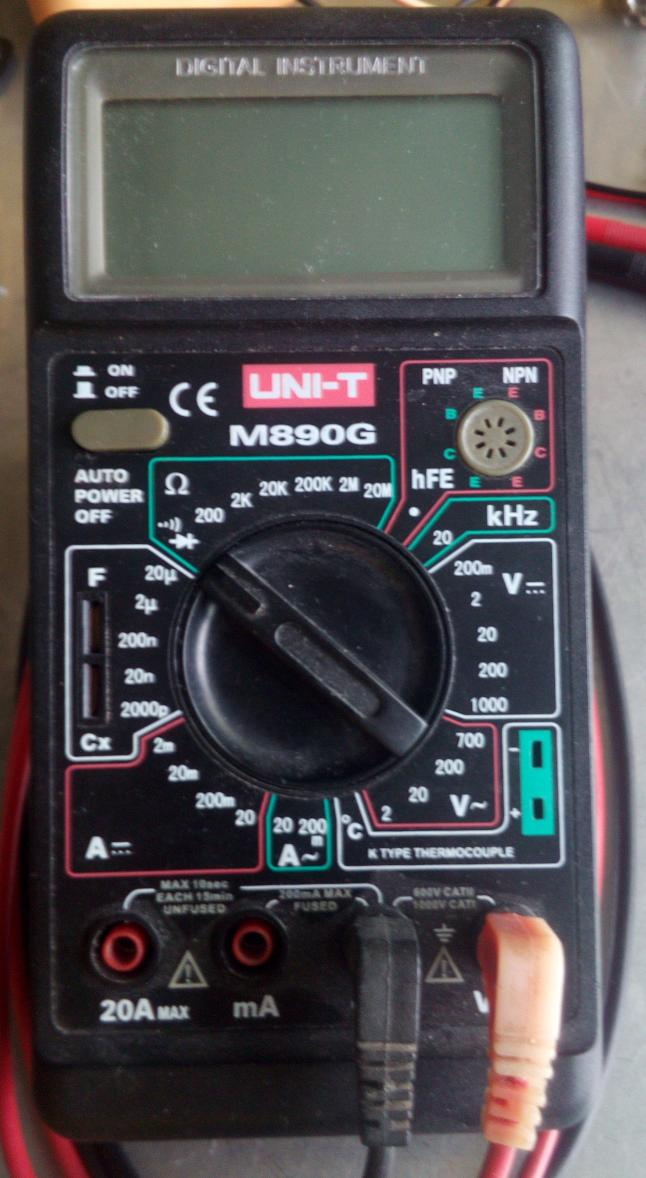
\includegraphics[width=6.5cm]{warsztat_elektroniczny/multimetr}\vspace{-1.2cm}\end{wrapfigure}
	\noindent
	Przydatne będą także funkcje takie jak:
	\begin{itemize}
		\item  sygnalizacja akustyczna ciągłości obwodu (może być razem z pomiarem diody)
		\item pomiar tranzystora "hfe"
	\end{itemize}
	Oczywiście fajnie jak nasz miernik będzie miał szersze zakresy pomiarowe, będzie umożliwiał pomiar prądu zmiennego (AC), pojemności kondensatorów, itd., ale nie jest to wymagane.
	
	Warto natomiast aby posiadał zabezpieczenie pomiaru prądu (czyli bezpiecznik w tym obwodzie, oznaczenie przy gniazdach "fused") przynajmniej na zakresie do 200mA.
	Natomiast przy teście diody warto aby miernik podawał napięcie wystarczające, jeżeli nie do zmierzenia, to przynajmniej do zaświecenia dowolnego LED (czyli tak naprawdę białego lub niebieskiego).
		Niestety producenci na ogół nie podają tego parametru i nawet dobre mierniki potrafią mieć ten paramter zaskakująco słaby.
	
	Ogólnie dobry multimetr jest ważny, ale na początek wystarczy nawet najtańszy model. Jeżeli będziemy kontynuować przygodę z elektroniką to z czasem i tak kupimy drugi, gdyż często przydaje się możliwość równoległego pomiaru w dwóch punktach, równoczesnego pomiaru prądu i napięcia, itd.
	
	\subsection{Propozycje}
	
	\subsubsection{DT-830B /  DT-830D / DT-832 / DT-832D} (jest wiele bardzo zbliżonych modeli – warto zwrócić uwagę aby miał "fused" na zakresie 200mA oraz buzzer do sygnalizacji ciągłości obwodu)
		\begin{itemize}
			\zaleta spełnia wymagania minimalne oraz posiada pomiar hfe i test ciągłości obwodu
			\zaleta pomiar napięcia DC i AC do 500V
			\zaleta pomiar prądu DC do 10A
			\info od 10PLN
		\end{itemize}

	\subsubsection{DT9205A}
		\begin{itemize}
			\zaleta spełnia wymagania minimalne oraz posiada pomiar hfe i test ciągłości obwodu
			\zaleta pomiar napięcia DC i AC do 500V
			\zaleta pomiar prądu DC i AC do 20A
			\zaleta pomiar pojemności
			\info od 20PLN
		\end{itemize}
	
	\subsubsection{DT33A} (nie mylić z DT33B, DT33C i DT33D):
		\begin{itemize}
			\zaleta spełnia wymagania minimalne oraz posiada pomiar hfe i test ciągłości obwodu
			\zaleta pomiar napięcia DC i AC do 500V
			\zaleta pomiar prądu DC do 10A
			\zaleta pomiar pojemności
			\zaleta pomiar temperatury
			\info od 30PLN
		\end{itemize}
	
	\subsubsection{DT890G / M890G / M890C}
		\begin{itemize}
			\zaleta spełnia wymagania minimalne oraz posiada pomiar hfe i test ciągłości obwodu
			\zaleta pomiar napięcia DC i AC do 500V
			\zaleta pomiar prądu DC i AC do 20A
			\zaleta pomiar pojemności
			\zaleta pomiar temperatury
			\zaleta pomiar częstotliwości (tylko DT890G / M890G)
			\zaleta (u niektórych producentów) zabezpieczony pomiar 20A
			\info od 35PLN
		\end{itemize}
	
	\subsubsection{Uni-T UT890C+}
		\begin{itemize}
			\zaleta spełnia wymagania minimalne oraz posiada pomiar hfe i test ciągłości obwodu
			\zaleta pomiar napięcia DC i AC do 500V
			\zaleta pomiar prądu DC i AC do 20A
			\zaleta pomiar pojemności
			\zaleta pomiar temperatury
			\zaleta pomiar częstotliwości
			\zaleta zabezpieczony pomiar 20A
			\zaleta zakresy 6, 60, 600 a nie 2, 20, 200
			\zaleta true RMS
			\info od 76PLN
		\end{itemize}

\section{Warsztat – płytka stykowa, przewody i śrubokręt}
	Kolejnymi rzeczami w które warto się zaopatrzyć są elementy umożliwiają łatwe budowanie układów prototypowych:
	\begin{itemize}
		\item płytka prototypowa stykowa (jedna lub dwie)
		\item przewody męsko-męskie (około 30sztuk)
		\item przewody męsko-żeńskie (około 10sztuk)
		\item przewody żeńskie-żeńskie (opcjonalnie, około 10sztuk)
		\item przewody pin męski - krokodylek lub krokodylek-krokodylek (około 5sztuk)
		\item śrubokręt mały płaski
	\end{itemize}
	
	\vspace{12pt}
	\hspace{\stretch{2}}
		\parbox[c]{0.45\textwidth}{
			\includegraphics[height=5.3cm]{warsztat_elektroniczny/płytka_i_przewody}\footnotesize
			\\na górze od lewej: przewód męsko-męski (czerwony), żeńsko-żeński (czarny) i męsko-żeński (żółty);
			\\poniżej przykładowa płytka stykowa
		}
	\hspace{\stretch{1}}
		\parbox[c]{0.45\textwidth}{
			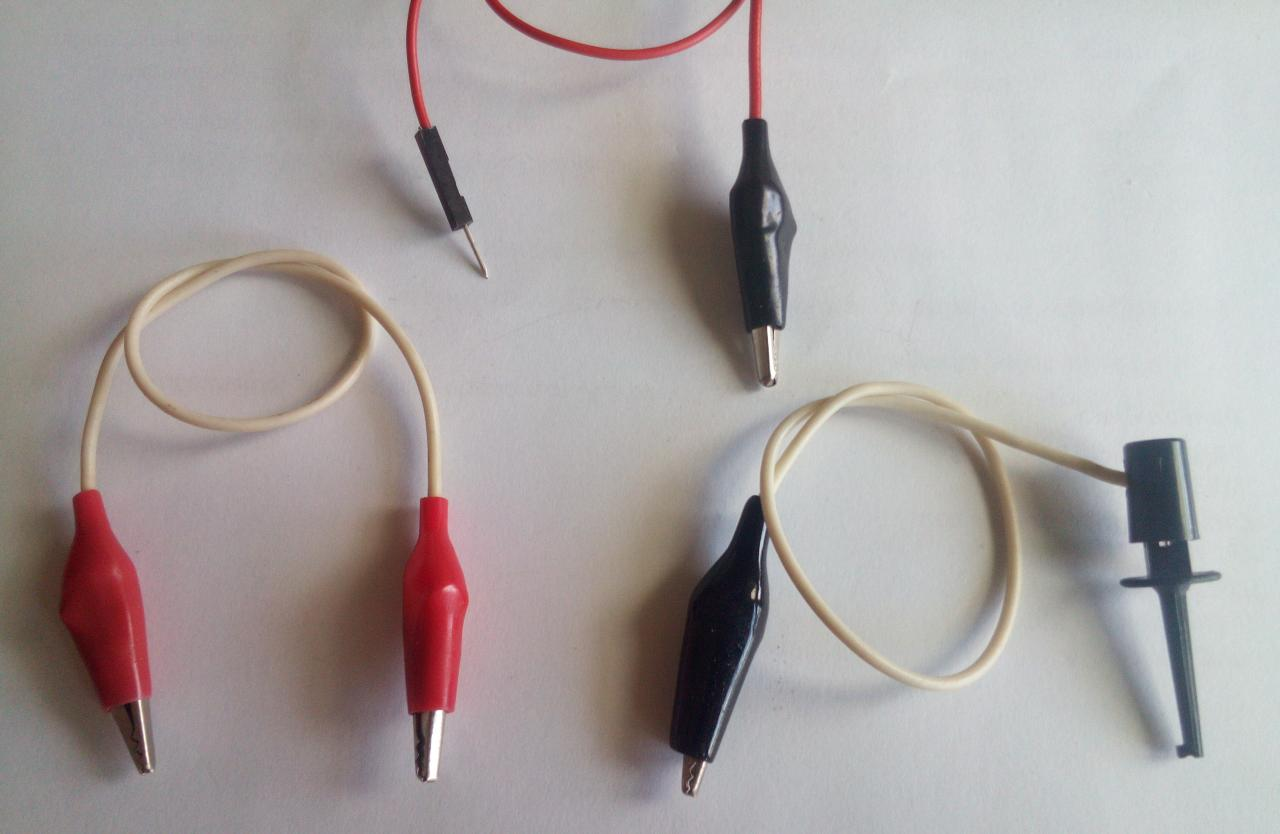
\includegraphics[height=5.3cm]{warsztat_elektroniczny/krokodylki}\footnotesize
			\\od lewej: przewód krokodylek - krokodylek (biało-czerwony), krokodylek - pin męski (czerwono-czarny), krokodylek - chwytak (biało-czarny)
		}
	\hspace{\stretch{2}}
	\vspace{12pt}
	
	Koszt płytki prototypowej, zestawu kabelków i śrubokręta to około 20PLN.

\section{Mikrokontroler i programator}

\subsection{Moduł STM32}
	\parbox[c]{0.55\textwidth}{
		W ramach zajęć będziemy uczyć się podstaw programowania mikrokontrolerów w oparciu o mikrokontroler STM32F103C8.
		W tym celu potrzebne będą nam płytka zawierająca mikrokontroler wraz niezbędnymi peryferiami - będziemy używać tzw. modułu „blue-pill” pokazanego na zdjęciu obok. Cena od około 11.5PLN.
	}
	\hspace{\stretch{1}}
	\parbox[c]{0.43\textwidth}{
		\begin{flushright} 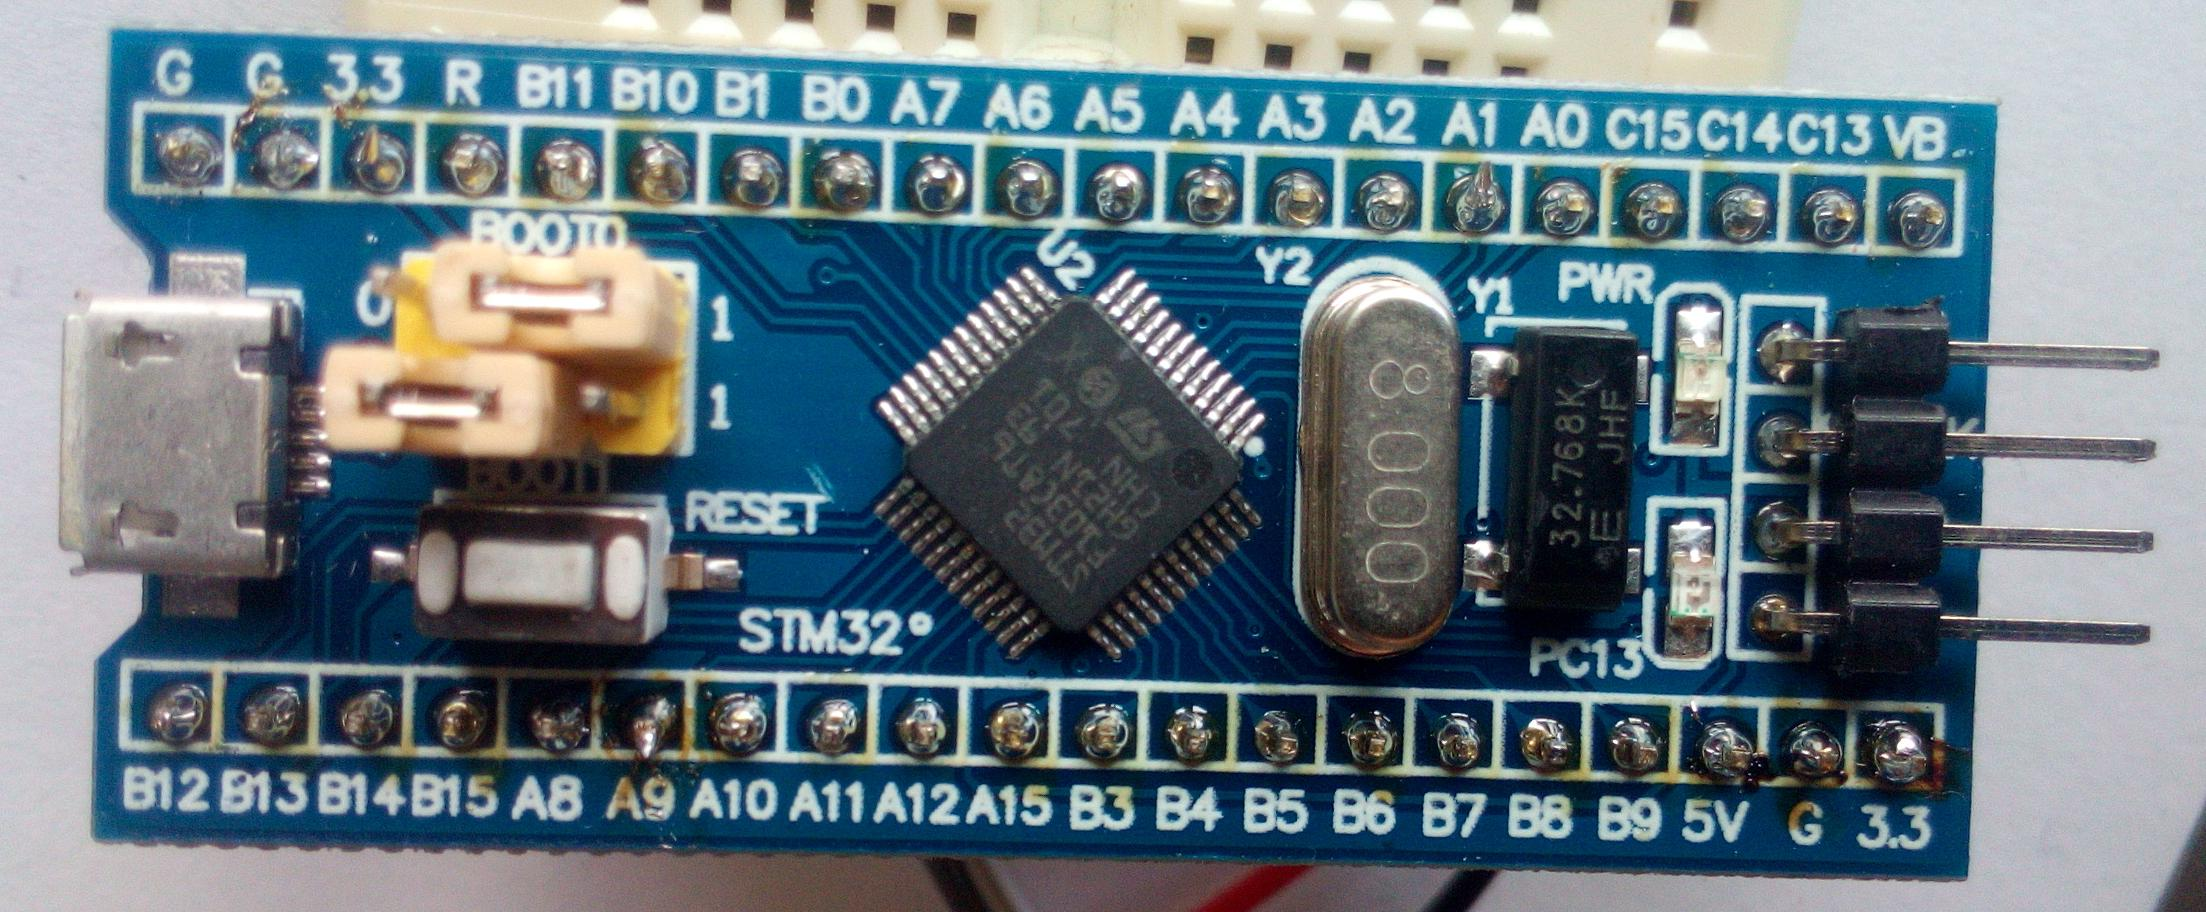
\includegraphics[height=3.3cm]{warsztat_elektroniczny/blue-pill} \end{flushright}
	}

\subsection{Konwerter USB-UART}
	Do programowania użyjemy portu szerowego naszego mikrokontrolera, w celu połączenia się z nim potrzebna będzie przejściówka USB-UART. Zasadniczo dowlna tego typu przejściówka (mająca napięcia logiczne na poziomie 3.3V, czyli \textbf{nie} przejściówka typu RS232) będzie OK. Poniżej dwie przetestowane propozycje do wyboru.
	
	\subsubsection{Moduł z układem PL2303HX}
	\parbox[c]{0.55\textwidth}{
		\begin{itemize}
			\wada moduł ma wyprowadzone jedynie linie RxD i TxD
			\wada moduł do wygodnego używania wymaga przedłużacza USB
			\info od 3.5PLN
		\end{itemize}
	}
	\hspace{\stretch{1}}
	\parbox[c]{0.43\textwidth}{
		\begin{flushright} 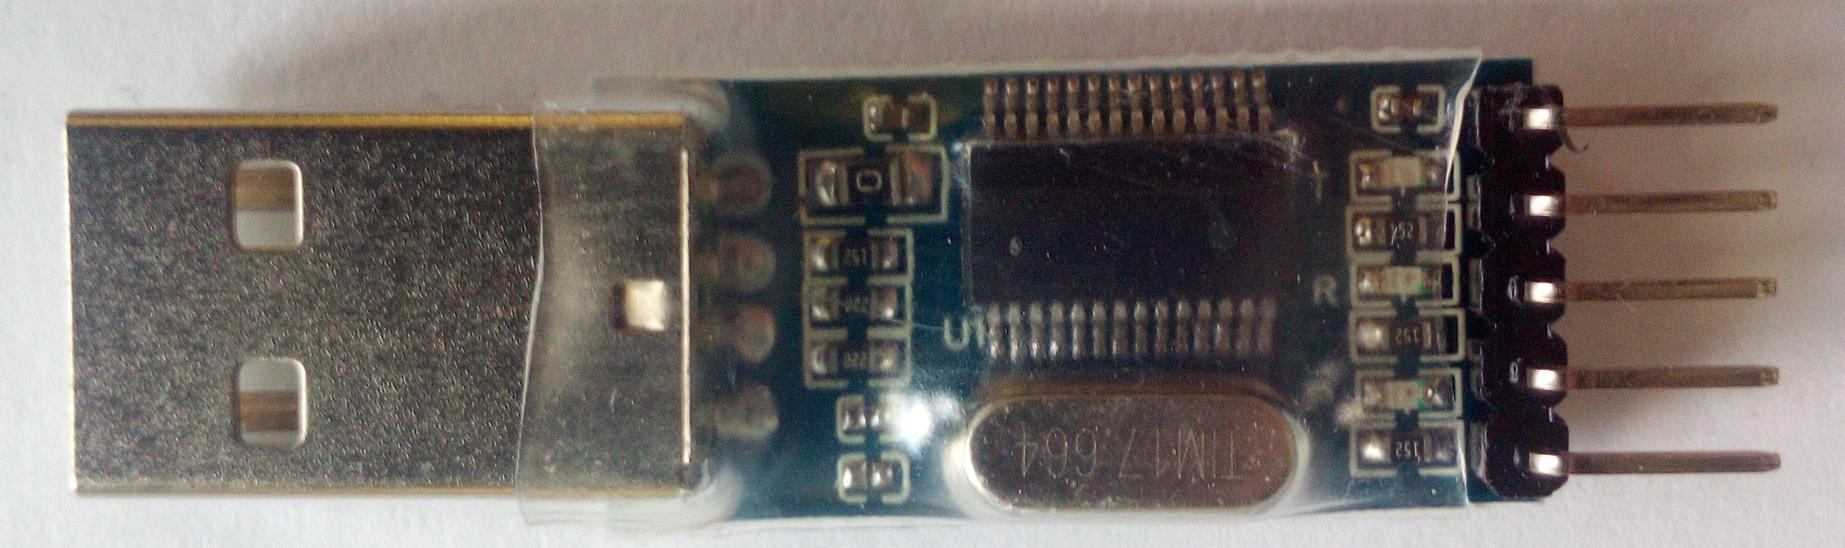
\includegraphics[height=2.3cm]{warsztat_elektroniczny/usb-uart1} \end{flushright}
	}
	
	\subsubsection{Moduł z układem FTDI FT232RL}
	\parbox[c]{0.65\textwidth}{
		\begin{itemize}
			\zaleta moduł ma wyprowadzone na bocznych wszystkie linie portu szeregowego, co prawda nam nie będzie to potrzebne, ale może się przydać w innych zastosowaniach (np. programowanie układów ESP)
			\wada moduł wymaga kabla mini-usb
			\info od 10PLN
		\end{itemize}
	}
	\hspace{\stretch{1}}
	\parbox[c]{0.33\textwidth}{
		\begin{flushright} 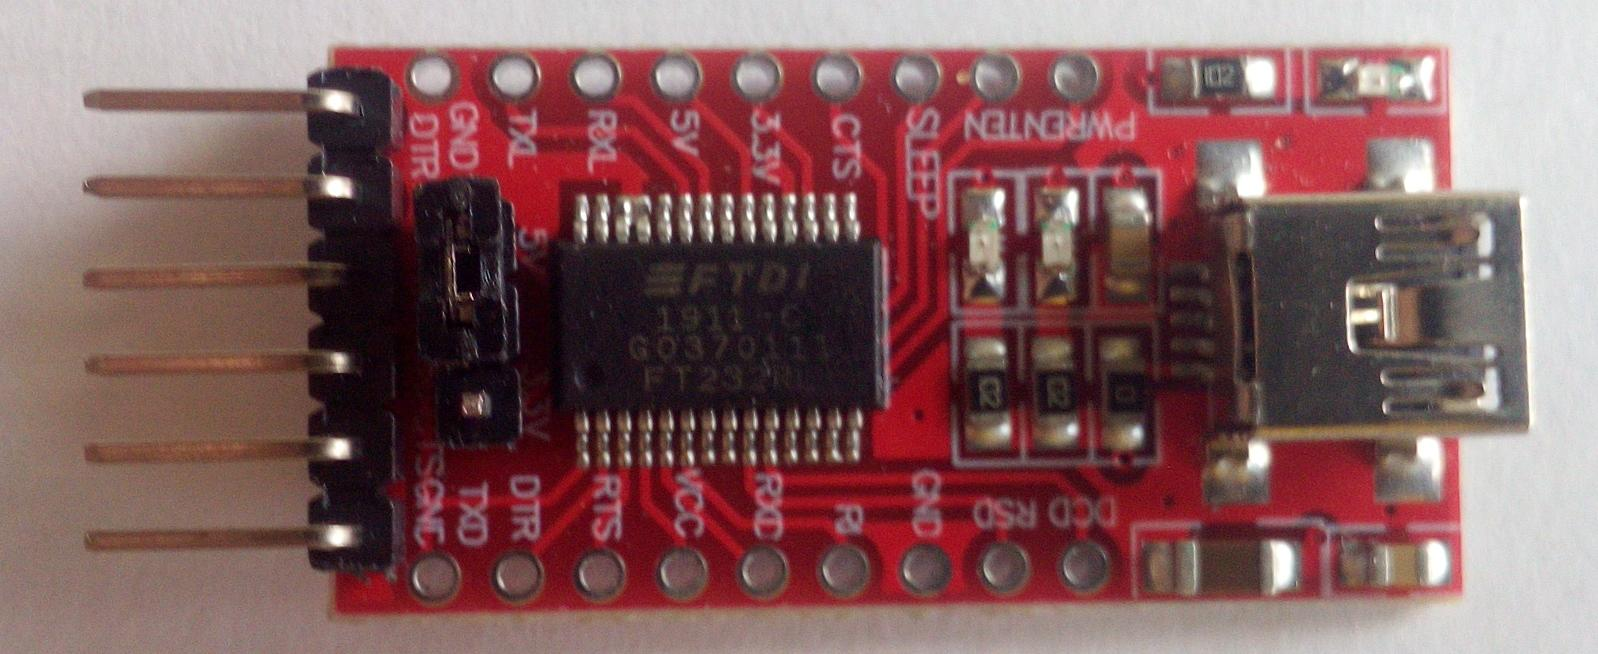
\includegraphics[height=2.3cm]{warsztat_elektroniczny/usb-uart2} \end{flushright}
	}
	
\section{Podzespoły elektroniczne}

Będzie potrzebny też zestaw drobnych podzespołów elektronicznych:
\begin{itemize}
	\item rezystory 1kΩ i 22kΩ, po około 10 sztuk
	\item potencjometr / rezystor nastwany 5kΩ, który da się włożyć w płytkę stykową, najlepiej wieloobrotowy, 1-2 sztuki
	\item kondensator elektrolityczny 100uF, kilka sztuk
	
	\item dioda prostownicza, około 10 sztuk
	\item dioda świecąca, około 10 sztuk
	\item tranzystor NPN (np. BC337) i PNP (np. BC327), po kilka sztuk
	
	\item układ logiczny z serii 4000 lub 7400: NAND (np. CD4011BE) lub NOR (np. CD4001BP)
	\item rejestr przesuwny z serii 4000 lub 7400 (np. CD4094 lub 74HC595)
\end{itemize}

\section{Inne}
Jeżeli kupiony moduł STM32 nie ma przylutowanych pinów po bokach (a na ogół nie ma), będzie potrzebna także lutownica z cyną i kalafonią. Koszt od 16PLN.

Oczywiście do programowania mikrokotrolera będzie potrzebny także działający komputer z portem USB i system Linux (to na nim będzie oparte nasze środowisko do tworzenia programów dla STM32), ale zakładamy że jakiś już masz {\Symbola 😄}.

\copyrightFooter{
	© Matematyka dla Ciekawych Świata, 2020.\\
	© Robert Ryszard Paciorek <rrp@opcode.eu.org>, 2020.\\
	Kopiowanie, modyfikowanie i redystrybucja dozwolone pod warunkiem zachowania informacji o autorach.
}

\end{document}
